\scanpage{79}
% archive sheet number: 78
Directions remarquables
\[
\begin{aligned}
\unsure{6}&\quad\text{directions de \unsure{sommet|sommets}}\\
15&\quad\text{--- d'arêtes}\\
\underline{10}&\quad\text{directions de faces}\\
31&=5^2+5+1\quad\text{nb de pts du plan projectif sur }\mathbb F_5
\end{aligned}
\]
Les 6 directions de \unsure{sommet|sommets} correspondent à la \unsure{conique}. Les \inserted{15} directions d'\deleted{\unsure{faces}}\inserted{arêtes} correspondent aux sécantes découpant un diviseur \deleted{$\unsure{\to}$}\inserted{\unsure{décomposé}}$/\mathbb F_5$ ; les \inserted{10} directions de faces correspondent aux diviseurs \unsure{connexes} $/\mathbb F_5$.

vecteurs remarquables en \uline{car. 5}
\[
1+12+60+40=11\deleted{\unsure{2}}3
\qquad
125=\underset{\infty}{1}+\underbrace{24}_{\substack{\text{pts sur}\\\text{la conique}\\=2\times12\\\text{(deux ico.)}}}+60+40
\]
\unsure{des|les} \deleted{\unsure{quinze}}\inserted{25} \unsure{droites|doubles} non isotropes

\deleted{\unsure{20}\ \unsure{points}}\inserted{15}\ \deleted{\unsure{plans}} associés aux \deleted{\unsure{arêtes}}\inserted{arêtes}\ \deleted{\unsure{les points}}\ \deleted{\unsure{dist.|distincts}}.

\deleted{\unsure{distingués}}

20 aux faces --- elles sont \inserted{\unsure{donc}}

\figure{%
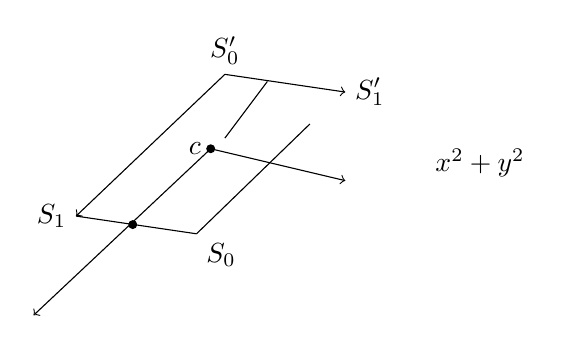
\begin{tikzpicture}[scale=.9]
\coordinate (s1) at (0,0);\coordinate(s0) at (1.7,-.25);
\coordinate(sp0) at (2.1,2);\coordinate(sp1) at (3.8,1.75);
\draw[->] (sp0)--(s1);\draw (s1)--(s0);\draw[->] (sp0)--(sp1);
\draw (2.7,1.9)--(2.1,1.1);\draw (s0)--(3.3,1.3);
\draw[->] (1.9,.95)--(-.6,-1.4);\draw[->] (1.9,.95)--(3.8,.5);
\fill (.8,-.12) circle(1.8pt);\fill(1.9,.95) circle(1.8pt);
\node[left] at(s1){$S_1$};\node[below right] at(s0){$S_0$};
\node[above] at(sp0){$S'_0$};\node[right] at(sp1){$S'_1$};
\node[left] at(1.9,.95){$c$};
\node at(5.7,.75){$\deleted{x^2+y^2}$};
\end{tikzpicture}}

% archive/scan mark: isolated right-angle registration-like mark near lower edge
